
\documentclass[11pt]{article}

\usepackage[paperwidth=8.5in,paperheight=11in,margin=0.72in,top=0.74in,bottom=0.78in]{geometry}
\usepackage[T1]{fontenc}
\usepackage[utf8]{inputenc}
\usepackage{newtxtext,newtxmath}
\usepackage{microtype}
\usepackage{amsmath,mathtools}
\usepackage{booktabs,tabularx,array,multirow}
\usepackage{graphicx}
\usepackage{enumitem}
\usepackage{tikz}
\usetikzlibrary{arrows.meta,positioning,calc,fit,backgrounds,shapes.geometric,shadows.blur}
\usepackage[most]{tcolorbox}
\usepackage{xcolor}
\usepackage{fancyhdr}
\usepackage{titlesec}
\usepackage{hyperref}
\usepackage{lastpage}
\usepackage{parskip}
\usepackage{ragged2e}
\usepackage{listings}
\usepackage{caption}
\usepackage{eso-pic}
\usepackage{pagecolor}

\definecolor{Ivory}{HTML}{FBF7EE}
\definecolor{Ink}{HTML}{101521}
\definecolor{Navy}{HTML}{162448}
\definecolor{Royal}{HTML}{2F3E85}
\definecolor{Violet}{HTML}{6B56CC}
\definecolor{Gold}{HTML}{B1841F}
\definecolor{SoftGold}{HTML}{EAD8A5}
\definecolor{PaleGold}{HTML}{FFF6D8}
\definecolor{Mint}{HTML}{DFF3EA}
\definecolor{Sky}{HTML}{E6F3F6}
\definecolor{Lavender}{HTML}{ECE9FF}
\definecolor{Rose}{HTML}{FBE6E9}
\definecolor{PaleBlue}{HTML}{EEF4FF}
\definecolor{Line}{HTML}{D8C9A1}
\definecolor{CodeBg}{HTML}{F6F2EA}
\pagecolor{Ivory}
\color{Ink}

\hypersetup{
  colorlinks=true,
  linkcolor=Royal,
  citecolor=Royal,
  urlcolor=Royal,
  pdftitle={PROOF_LOOPS.md: Field Notes on Machines That Turn Work Into Capability},
  pdfauthor={Vincent Boucher},
  pdfsubject={GoalOS proof-gated autonomous work loops},
  pdfkeywords={GoalOS, Proof Loops, Validated Skill Graph, AGI Jobs, Evidence Docket, Chronicle, proof economy}
}

\setlength{\parskip}{0.52em}
\setlength{\parindent}{0pt}
\setlength{\headheight}{22pt}
\emergencystretch=2em
\setlist[itemize]{leftmargin=1.2em,itemsep=0.18em,topsep=0.2em}
\setlist[enumerate]{leftmargin=1.45em,itemsep=0.18em,topsep=0.2em}
\captionsetup{font=small,labelfont={bf,color=Navy},textfont=it,skip=6pt}

\pagestyle{fancy}
\fancyhf{}
\fancyhead[L]{\small\scshape PROOF\_LOOPS.md}
\fancyhead[C]{\small\color{Gold}\ensuremath{\diamond}}
\fancyhead[R]{\small\scshape Vincent Boucher}
\fancyfoot[L]{\small\color{Navy}QUEBEC.AI \& MONTREAL.AI}
\fancyfoot[R]{\small\thepage\,/\,\pageref*{LastPage}}
\renewcommand{\headrulewidth}{0.35pt}
\renewcommand{\footrulewidth}{0pt}
\renewcommand{\headrule}{\hbox to\headwidth{\color{Line}\leaders\hrule height \headrulewidth\hfill}}

\titleformat{\section}{\Large\bfseries\scshape\color{Navy}}{\thesection}{0.7em}{}[\vspace{-0.35em}\color{Gold}\titlerule]
\titleformat{\subsection}{\large\bfseries\color{Navy}}{\thesubsection}{0.55em}{}
\titleformat{\subsubsection}{\normalsize\bfseries\color{Navy}}{\thesubsubsection}{0.5em}{}

\tcbset{enhanced,boxsep=4pt,arc=5pt,outer arc=5pt,boxrule=0.6pt,left=8pt,right=8pt,top=7pt,bottom=7pt}
\newtcolorbox{lawbox}[1]{colback=PaleGold,colframe=Gold,title={#1},fonttitle=\bfseries\scshape,coltitle=Ink}
\newtcolorbox{bluebox}[1]{colback=PaleBlue,colframe=Royal,title={#1},fonttitle=\bfseries\scshape,coltitle=Ink}
\newtcolorbox{greenbox}[1]{colback=Mint,colframe=teal!55!black,title={#1},fonttitle=\bfseries\scshape,coltitle=Ink}
\newtcolorbox{redbox}[1]{colback=Rose,colframe=red!55!black,title={#1},fonttitle=\bfseries\scshape,coltitle=Ink}
\newtcolorbox{notebox}[1]{colback=Ivory,colframe=Line,title={#1},fonttitle=\bfseries\scshape,coltitle=Ink}

\lstdefinestyle{jsonstyle}{
  backgroundcolor=\color{CodeBg},
  basicstyle=\ttfamily\small,
  breaklines=true,
  columns=fullflexible,
  frame=single,
  rulecolor=\color{Line},
  xleftmargin=0pt,
  xrightmargin=0pt,
  showstringspaces=false,
  keepspaces=true
}
\lstset{style=jsonstyle}

\tikzset{
  flow/.style={rounded corners=7pt, draw=Royal!65, fill=white, very thick, align=center, inner sep=6pt, minimum height=0.52in, text width=0.83in, font=\scriptsize\bfseries},
  flowgold/.style={flow, draw=Gold!70!black, fill=PaleGold},
  flowgreen/.style={flow, draw=teal!65!black, fill=Mint},
  flowrose/.style={flow, draw=red!60!black, fill=Rose},
  flowsky/.style={flow, draw=cyan!50!black, fill=Sky},
  arrow/.style={-{Stealth[length=2.4mm]}, very thick, draw=Royal!82},
  darrow/.style={-{Stealth[length=2.4mm]}, thick, dashed, draw=Gold!80!black},
  faint/.style={draw=Line, rounded corners=8pt, fill=white, fill opacity=0.72, text opacity=1},
  layer/.style={rounded corners=7pt, draw=Navy!60, fill=white, very thick, align=left, inner sep=8pt, text width=6.4in, minimum height=0.55in},
  mini/.style={rounded corners=6pt, draw=Royal!55, fill=white, align=center, inner sep=5pt, font=\scriptsize\bfseries, minimum height=0.38in},
  tag/.style={rounded corners=4pt, draw=Gold!70!black, fill=PaleGold, align=center, inner sep=4pt, font=\scriptsize\bfseries}
}

\newcommand{\doccode}[1]{\texttt{#1}}
\newcommand{\GoalOS}{\textsc{GoalOS}}
\newcommand{\Chronicle}{\textsc{Chronicle}}
\newcommand{\VSG}{\textsc{Validated Skill Graph}}
\newcommand{\ProofBundle}{\textsc{ProofBundle}}
\newcommand{\EvidenceDocket}{\textsc{Evidence Docket}}
\newcommand{\AGIJobs}{\textsc{AGI Jobs}}

\begin{document}

% Title page
\begin{titlepage}
\thispagestyle{empty}
\AddToShipoutPictureBG*{%
\begin{tikzpicture}[remember picture,overlay]
  \fill[Ivory] (current page.south west) rectangle (current page.north east);
  \draw[Gold!25, line width=0.7pt] ($(current page.center)+(-3.45,-4.85)$) circle (2.35);
  \draw[Royal!15, line width=0.7pt] ($(current page.center)+(-3.45,-4.85)$) circle (3.05);
  \draw[cyan!20, dashed, line width=0.7pt] ($(current page.center)+(-3.45,-4.85)$) circle (2.7);
  \draw[Gold!18, line width=0.8pt] ($(current page.north west)+(0.55,-0.55)$) -- ($(current page.north east)+(-0.55,-0.55)$);
  \draw[Gold!18, line width=0.8pt] ($(current page.south west)+(0.55,0.55)$) -- ($(current page.south east)+(-0.55,0.55)$);
  \fill[Royal!5] ($(current page.north east)+(-1.3,-1.65)$) circle (0.7);
  \fill[Gold!9] ($(current page.south east)+(-1.7,2.0)$) circle (1.0);
\end{tikzpicture}}
\vspace*{0.45in}
\begin{center}
{\small\scshape\color{Gold} Montreal.AI Research \quad \ensuremath{\diamond} \quad GoalOS Protocol Note Series}\par
\vspace{0.78in}
{\fontsize{29}{32}\selectfont\bfseries\color{Navy} PROOF\_LOOPS.md}\par
\vspace{0.18in}
{\fontsize{20}{24}\selectfont\bfseries Field Notes on Machines That Turn Work Into Capability}\par
\vspace{0.2in}
{\Large\itshape A research architecture for proof-gated autonomous work, Chronicle memory,\par and on-chain graph-root commitments}\par
\vspace{0.45in}
{\color{Gold}\rule{3.8in}{0.6pt}}\par
\vspace{0.36in}
{\large\bfseries Vincent Boucher}\par
{\normalsize President, QUEBEC.AI \& MONTREAL.AI}\par
\vspace{0.2in}
{\small Research Edition v2.0 \quad | \quad Publication-safe, claim-bounded}\par
\end{center}
\vfill
\begin{lawbox}{Core loop}
\centering
\Large
Objective $\rightarrow$ Proof Mission $\rightarrow$ AGI Jobs $\rightarrow$ Evidence $\rightarrow$ Chronicle $\rightarrow$ Validated Skill $\rightarrow$ On-chain Graph Root $\rightarrow$ Future Mission Improvement
\end{lawbox}
\vspace{0.35in}
\begin{center}
\small\itshape
AI creates output. GoalOS creates proof. The machine may draft; the institution must decide what earns memory.
\end{center}
\end{titlepage}
\ClearShipoutPictureBG

\begin{abstract}
\noindent \doccode{PROOF\_LOOPS.md} specifies a compact operating law for proof-gated autonomous work: an objective becomes a proof mission; proof debt becomes AGI Jobs; jobs return evidence; evidence is gated by Chronicle; validated skills become graph memory; graph roots can be committed on-chain; and admitted skills improve future missions. This paper converts that operating note into a formal research architecture. It defines a state model, proof-debt mechanics, AGI Job contracts, Evidence Dockets, Chronicle admission, Validated Skill Graph accumulation, proof-level policy, on-chain commitment boundaries, and falsification tests. The central claim is architectural and testable: durable autonomy requires proof-carrying loops that prevent unverified output from becoming institutional memory. The paper does not claim achieved AGI, achieved ASI, legal certification, financial advice, production authorization, live settlement, or external validation. It defines the loop required for such claims to become inspectable, replayable, and governed.
\end{abstract}

\begin{center}
\small\textbf{Keywords:} GoalOS; proof loops; autonomous agents; Proof Debt; AGI Jobs; Evidence Dockets; Chronicle; Validated Skill Graph; on-chain commitments; proof economy.
\end{center}

\begin{lawbox}{Executive thesis}
A prompt is a request. A proof loop is an institution. The prompt asks a model to answer; the loop decides what must be proven before the answer can matter.
\end{lawbox}

\section{Introduction}
Frontier models make candidate work abundant. They produce claims, reports, code, plans, critiques, tool traces, and agent outputs at low marginal cost. The institutional problem is not whether an AI system can generate. It is whether a result deserves trust, reuse, payment, propagation, memory, or rollback authority.

\GoalOS{} answers by separating output from authority. Model output is candidate work. Candidate work may create Proof Debt. Proof Debt may become AGI Jobs. Jobs may return \ProofBundle{} artifacts. Those artifacts may update an \EvidenceDocket{}. Only then can \Chronicle{} decide whether a capability enters durable memory as a validated skill.

The note \doccode{PROOF\_LOOPS.md} compresses the system to one loop:
\[
\begin{aligned}
\text{Objective} &\rightarrow \text{Proof Mission} \rightarrow \text{AGI Jobs} \rightarrow \text{Evidence} \rightarrow \text{Chronicle}\\
&\rightarrow \text{Validated Skill} \rightarrow \text{On-chain Graph Root} \rightarrow \text{Future Mission Improvement}.
\end{aligned}
\]
This paper gives that loop a research form: objects, transition rules, gates, proof levels, privacy boundary, threat model, and evaluation program.

\section{Contributions}
This paper makes seven contributions.
\begin{enumerate}
  \item \textbf{Proof-loop formalism.} A state-machine model for converting objectives into proof-gated capability.
  \item \textbf{Proof Debt to AGI Job conversion.} A job factory that starts empty and creates only the proof work required by the mission.
  \item \textbf{Evidence Docket model.} A structured proof room that turns artifacts into inspectable claims, risks, replay paths, and validator records.
  \item \textbf{Chronicle admission law.} A memory firewall preventing unsupported output from influencing future missions.
  \item \textbf{Validated Skill Graph accumulation.} A capability graph that stores scoped, replayable, evidence-backed skills rather than prompt fragments.
  \item \textbf{On-chain graph-root boundary.} A public/private model in which private intelligence remains protected while proof commitments can be anchored.
  \item \textbf{Falsification program.} Tests for whether proof loops outperform report-only, prompt-library, and ungated-agent baselines.
\end{enumerate}

\begin{figure}[p]
\centering
\resizebox{0.985\textwidth}{!}{%
\begin{tikzpicture}[node distance=0.18in]
\node[flowgold] (o) {1\\Objective};
\node[flow, right=0.14in of o] (pm) {2\\Proof\\Mission};
\node[flowrose, right=0.14in of pm] (j) {3\\AGI\\Jobs};
\node[flowsky, right=0.14in of j] (e) {4\\Evidence};
\node[flow, right=0.14in of e] (c) {5\\Chronicle};
\node[flowgreen, right=0.14in of c] (s) {6\\Validated\\Skill};
\node[flowgold, right=0.14in of s] (r) {7\\On-chain\\Root};
\node[flowgreen, right=0.14in of r] (f) {8\\Future\\Mission};
\foreach \a/\b in {o/pm,pm/j,j/e,e/c,c/s,s/r,r/f} \draw[arrow] (\a) -- (\b);
\draw[darrow] (f.south) .. controls +(0,-0.55) and +(0,-0.55) .. node[below, font=\scriptsize\itshape, yshift=-2pt]{capability prior only from admitted skill} (o.south);
\node[flowrose, below=0.75in of j] (d) {Proof\\Debt};
\draw[darrow] (e.south) .. controls +(0,-0.3) and +(0,-0.3) .. node[below, font=\scriptsize]{incomplete proof} (d.south);
\draw[arrow] (d) -- (j);
\node[tag, below=0.35in of s, text width=4.4in] (law) {Loop law: work does not become memory until evidence passes Chronicle.};
\end{tikzpicture}%
}
\caption{The canonical proof loop. The loop turns autonomous work into proof, proof into validated skill, skill into graph memory, and graph memory into future mission improvement.}
\label{fig:coreloop}
\end{figure}

\section{System Doctrine}
The proof loop rests on four doctrines.

\begin{greenbox}{Doctrine 1: output is not authority}
A model may answer; an agent may act; an institution must prove. Fluency cannot grant future mission influence.
\end{greenbox}

\begin{greenbox}{Doctrine 2: memory is gated}
No Chronicle entry means no future mission influence. Memory must be admitted, scoped, replayable, and rollbackable.
\end{greenbox}

\begin{greenbox}{Doctrine 3: work is proof-producing}
AGI Jobs are not tasks in a todo list. They are proof contracts with claim, worker, validator, acceptance tests, blocked claims, and ProofBundle return path.
\end{greenbox}

\begin{greenbox}{Doctrine 4: public proof, private intelligence}
Do not expose private skill intelligence as plaintext. Use commitments, encrypted capsules, attestations, and zero-knowledge proofs where applicable.
\end{greenbox}

\section{Formal State Model}
Let a proof-loop run at time $t$ have state
\begin{equation}
S_t=(O,M,C,D,J,P,E,V,K,R,F),
\end{equation}
where $O$ is the objective, $M$ the Mission Contract, $C$ the claim set, $D$ the Proof Debt register, $J$ the AGI Job queue, $P$ the returned ProofBundles, $E$ the Evidence Docket, $V$ the verifier state, $K$ the Chronicle decision state, $R$ the on-chain graph-root record, and $F$ the future mission prior.

A transition is
\begin{equation}
S_{t+1}=\tau(S_t,u_t,\pi_\ell,\rho_t),
\end{equation}
where $u_t$ is an operator or system action, $\pi_\ell$ is the selected proof-level policy, and $\rho_t$ is a review, replay, validation, or risk signal.

The loop is complete when
\begin{equation}
\operatorname{Done}(S_t)= M \wedge D_{retired} \wedge P \wedge E \wedge V_{pass} \wedge K_{decision} \wedge B_{boundary},
\end{equation}
where $B_{boundary}$ asserts that claim, privacy, wallet, settlement, and scope boundaries remain intact.

\section{Layered Architecture}
The proof loop is a layered operating system. Each layer narrows authority.

\begin{figure}[p]
\centering
\resizebox{0.985\textwidth}{!}{%
\begin{tikzpicture}[node distance=0.12in]
\node[layer, fill=PaleGold] (l1) {\textbf{1. Objective Layer} \\ User intent, decision to support, success criteria, failure criteria, constraints.};
\node[layer, below=0.10in of l1, fill=PaleBlue] (l2) {\textbf{2. Mission Layer} \\ Mission Contract, proof level, claim boundary, allowed tools, validators, rollback obligations.};
\node[layer, below=0.10in of l2, fill=Rose] (l3) {\textbf{3. Proof Layer} \\ Claim extraction, Proof Debt, custom AGI Jobs, worker/validator/sentinel assignments.};
\node[layer, below=0.10in of l3, fill=Sky] (l4) {\textbf{4. Evidence Layer} \\ ProofBundles, Evidence Docket, replay manifests, risk ledger, source provenance.};
\node[layer, below=0.10in of l4, fill=Lavender] (l5) {\textbf{5. Memory Layer} \\ Chronicle Gate, validated skill admission, Validated Skill Graph, future mission influence.};
\node[layer, below=0.10in of l5, fill=Mint] (l6) {\textbf{6. Commitment Layer} \\ On-chain graph roots, evidence roots, ProofBundle roots, policy hashes, attestations, encrypted capsule commitments.};
\foreach \a/\b in {l1/l2,l2/l3,l3/l4,l4/l5,l5/l6} \draw[arrow] ($ (\a.south)+(0,-0.02) $) -- ($ (\b.north)+(0,0.02) $);
\node[tag, below=0.16in of l6, text width=5.9in] {Authority increases only downward: objective to proof, proof to memory, memory to commitment. A failed gate returns the run to Proof Debt.};
\end{tikzpicture}%
}
\caption{Layered proof-loop architecture. GoalOS separates user objective, mission design, proof production, evidence validation, memory admission, and public commitment.}
\label{fig:layered}
\end{figure}

\section{Proof Mission and Mission Contract}
A Proof Mission is the conversion of an objective into an evidence-generating run. Its contract is the first authority-bearing object.

\begin{lstlisting}[caption={Mission Contract skeleton.}]
{
  "mission_id": "mission-001",
  "objective": "...",
  "decision_to_support": "...",
  "success_criteria": [],
  "failure_criteria": [],
  "constraints": [],
  "proof_level": "L3 External Review",
  "risk_class": "medium",
  "allowed_tools": [],
  "required_validators": [],
  "blocked_claims": [],
  "rollback_obligations": []
}
\end{lstlisting}

The mission contract prevents an agent from optimizing an ambiguous request. It states what the work is for, what would count as success, what would fail the mission, and which claims are blocked before proof.

\section{Proof Debt}
Proof Debt is the difference between what the system wants to claim and what it can support.

\begin{equation}
D_{proof}=\sum_i \operatorname{Impact}(c_i)\cdot \operatorname{Unsupported}(c_i)\cdot \operatorname{Irreversibility}(c_i)\cdot \operatorname{ReuseRisk}(c_i).
\end{equation}

A claim may be classified as supported, needs evidence, needs replay, needs reviewer, needs boundary, blocked, or out of scope. This turns uncertainty into a work queue rather than burying it in prose.

\section{Custom AGI Jobs}
The AGI Job factory starts empty. Jobs are generated only after the mission and proof level are known.

\begin{figure}[p]
\centering
\resizebox{0.985\textwidth}{!}{%
\begin{tikzpicture}[node distance=0.17in]
\node[flowgold, text width=1.0in] (obj) {Objective\\+ proof level};
\node[flow, right=0.28in of obj, text width=1.0in] (claims) {Claim\\boundary};
\node[flowrose, right=0.28in of claims, text width=1.0in] (debt) {Proof Debt\\register};
\node[flow, right=0.28in of debt, text width=1.0in] (factory) {Custom Job\\Factory};
\foreach \a/\b in {obj/claims,claims/debt,debt/factory} \draw[arrow] (\a) -- (\b);
\node[mini, below=0.55in of factory, xshift=-2.6in, text width=1.15in, fill=Sky] (evidence) {Evidence\\collection};
\node[mini, right=0.18in of evidence, text width=1.15in, fill=Sky] (replay) {Replay\\construction};
\node[mini, right=0.18in of replay, text width=1.15in, fill=Sky] (review) {Reviewer\\validation};
\node[mini, right=0.18in of review, text width=1.15in, fill=Sky] (boundary) {Boundary\\audit};
\foreach \n in {evidence,replay,review,boundary} \draw[arrow] (factory.south) |- (\n.north);
\node[flowgreen, below=0.72in of replay, text width=1.1in] (pb) {Returned\\ProofBundles};
\node[flowgreen, right=0.34in of pb, text width=1.15in] (skill) {Candidate\\Skill Capsule};
\draw[arrow] (evidence.south) |- (pb.west);
\draw[arrow] (replay.south) -- (pb.north);
\draw[arrow] (review.south) |- (pb.east);
\draw[arrow] (boundary.south) |- (skill.east);
\draw[arrow] (pb) -- (skill);
\node[tag, below=0.35in of pb, xshift=1.0in, text width=5.5in] {Empty-by-design rule: no jobs exist before the objective and proof level are set.};
\end{tikzpicture}%
}
\caption{Proof Debt becomes custom AGI Jobs. The workbench is empty until the mission defines claims, proof level, and boundary.}
\label{fig:jobfactory}
\end{figure}

An AGI Job is a proof contract:
\begin{lstlisting}[caption={AGI Job skeleton.}]
{
  "job_id": "agi-job-001",
  "proof_debt_id": "debt-001",
  "source_claim": "...",
  "worker": "Reviewer Agent or Human Reviewer",
  "validator": "AGI Node Validator + Human Review",
  "sentinel": "Boundary Sentinel",
  "deliverables": [],
  "acceptance_tests": [],
  "blocked_claims": [],
  "proofbundle_return_path": "proofbundles/agi-job-001.json",
  "status": "ready-for-execution"
}
\end{lstlisting}

\section{Evidence Docket}
The \EvidenceDocket{} is not a file pile. It is the proof room. It ties claims to sources, ProofBundles, validator verdicts, risk, replay, and decision state.

\begin{notebox}{Minimum docket contents}
Mission Contract; claims matrix; Proof Debt Register; ProofBundle manifest; source provenance; replay manifest; risk ledger; blocked claims; validator notes; Chronicle recommendation; rollback conditions.
\end{notebox}

A docket is complete only if a reviewer can answer: What was attempted? What evidence exists? What failed? What remains blocked? What may be reused? What must not be claimed?

\section{Chronicle Gate}
\Chronicle{} is the memory firewall. It admits only candidates that satisfy the selected proof level.

\begin{equation}
\operatorname{Admit}(c,\ell)=\mathbf{1}\{E(c)\geq\theta_E^\ell \wedge R(c)\leq\theta_R^\ell \wedge V(c)\geq\theta_V^\ell \wedge P(c)=1 \wedge B(c)=1\},
\end{equation}
where $E$ measures evidence strength, $R$ risk, $V$ validation coverage, $P$ replay readiness, and $B$ boundary compliance.

\begin{figure}[p]
\centering
\resizebox{0.985\textwidth}{!}{%
\begin{tikzpicture}[node distance=0.22in]
\node[flow, text width=1.0in] (cand) {Candidate\\Skill};
\node[flow, right=0.40in of cand, text width=1.0in] (docket) {Evidence\\Docket};
\node[diamond, aspect=1.45, draw=Gold!80!black, fill=PaleGold, very thick, align=center, font=\scriptsize\bfseries, right=0.48in of docket, inner sep=2pt, text width=0.82in] (gate) {Chronicle\\Gate};
\node[flowgreen, above right=0.28in and 0.48in of gate, text width=1.05in] (admit) {Admit\\memory entry};
\node[flowgold, right=0.48in of gate, text width=1.05in] (repair) {Repair\\AGI Jobs};
\node[flowrose, below right=0.28in and 0.48in of gate, text width=1.05in] (reject) {Reject /\\Quarantine};
\draw[arrow] (cand) -- (docket);
\draw[arrow] (docket) -- (gate);
\draw[arrow] (gate) -- node[above, font=\scriptsize]{pass} (admit);
\draw[darrow] (gate) -- node[above, font=\scriptsize]{missing proof} (repair);
\draw[darrow] (gate) -- node[below, font=\scriptsize]{policy fail} (reject);
\node[mini, above=0.48in of docket, fill=white] (support) {support};
\node[mini, below=0.48in of docket, fill=white] (replay) {replay};
\node[mini, above=0.48in of gate, fill=white] (valid) {validation};
\node[mini, below=0.48in of gate, fill=white] (risk) {risk};
\draw[darrow] (support) -- (gate);
\draw[darrow] (replay) -- (gate);
\draw[darrow] (valid) -- (gate);
\draw[darrow] (risk) -- (gate);
\node[tag, below=1.0in of gate, text width=5.9in] {Gate law: evidence becomes authority only through policy.};
\end{tikzpicture}%
}
\caption{Chronicle admission. A candidate skill can be admitted, repaired, rejected, or quarantined; unsupported candidates do not become future mission memory.}
\label{fig:chronicle}
\end{figure}

\section{Validated Skill Graph}
A validated skill is a governed capability object. It is scoped, evidenced, replayable, versioned, and rollbackable.

\begin{equation}
 s = \langle id,type,scope,method,evidence,tests,validators,risk,policy,version,rollback,utility\rangle.
\end{equation}

The graph $G_t=(V_t,E_t)$ contains skill nodes and policy-scoped edges. Edge types include reuse, compose, teach, package, audit, supersede, retire, and future-prior. A future mission may use a skill only if the mission context matches the skill's scope and proof level.

\begin{figure}[p]
\centering
\resizebox{0.985\textwidth}{!}{%
\begin{tikzpicture}[node distance=0.18in]
\node[circle, draw=Navy!65, fill=white, very thick, align=center, minimum size=1.15in, font=\scriptsize\bfseries] (skill) {Validated\\Skill\\Node};
\node[mini, left=1.05in of skill, yshift=0.85in, fill=PaleBlue, text width=1.25in] (scope) {Identity \& Scope\\id, type, limits};
\node[mini, left=1.05in of skill, yshift=0.20in, fill=Sky, text width=1.25in] (method) {Method \& Replay\\procedure, tests};
\node[mini, left=1.05in of skill, yshift=-0.45in, fill=Rose, text width=1.25in] (risk) {Risk Ledger\\misuse, drift};
\node[mini, right=1.05in of skill, yshift=0.85in, fill=Mint, text width=1.25in] (evidence) {Evidence\\bundles, docket};
\node[mini, right=1.05in of skill, yshift=0.20in, fill=Lavender, text width=1.25in] (validators) {Validators\\human, node};
\node[mini, right=1.05in of skill, yshift=-0.45in, fill=PaleGold, text width=1.25in] (policy) {Policy\\proof, version};
\foreach \n in {scope,method,risk,evidence,validators,policy} \draw[arrow] (\n) -- (skill);
\node[flowgreen, below=0.7in of skill, text width=1.25in] (mem) {Chronicle\\Memory};
\draw[arrow] (skill) -- (mem);
\node[flowgold, below left=0.42in and 1.4in of skill, text width=1.2in] (repair) {Repair Jobs\\if proof missing};
\node[flowrose, below right=0.42in and 1.4in of skill, text width=1.2in] (retire) {Retire /\\Rollback};
\draw[darrow] (skill) -- (repair);
\draw[darrow] (skill) -- (retire);
\node[tag, below=0.3in of mem, text width=5.8in] {Object law: a skill is not a note. It is a capability record with evidence, scope, replay, policy, and rollback.};
\end{tikzpicture}%
}
\caption{Validated skill object model. The skill carries operational semantics, proof, policy, and rollback, not merely text.}
\label{fig:skillnode}
\end{figure}

\section{Proof Levels}
Proof levels calibrate authority. A high-risk public claim, a mainnet handoff, and an exploratory draft should not share one proof threshold.

\begin{table}[h]
\centering
\small
\begin{tabularx}{\textwidth}{@{}p{0.55in}p{1.25in}X p{1.6in}@{}}
\toprule
Level & Name & Required posture & Memory effect \\
\midrule
L1 & Structural / Demo & Mission structure, explicit Proof Debt, local artifact coherence. & No durable Chronicle influence. \\
L2 & Internal Review & Operator or internal reviewer confirms usefulness, scope, and obvious safety. & Temporary reuse, clearly labeled. \\
L3 & External Review & Cross-source support or independent reviewer / AGI Node validation. & Scoped reusable skill. \\
L4 & Mainnet Handoff & Handoff packet with validated evidence, job specification, and settlement boundary. & May inform external execution preparation. \\
L5 & Chronicle / Formal & Multi-validator evidence, replay, baseline comparison, risk gate, rollback condition. & Durable future mission influence. \\
\bottomrule
\end{tabularx}
\caption{Proof levels. Higher levels increase validator burden, evidence strictness, replay duty, and authority.}
\label{tab:prooflevels}
\end{table}

The selected proof level is a mission parameter, not a label added after the fact. It controls job decomposition, validator density, Evidence Docket strictness, and Chronicle threshold.

\section{On-chain Graph Root and Privacy Boundary}
The on-chain graph root is a public commitment, not the skill itself. The skill lives in the encrypted capsule, Evidence Docket, ProofBundles, replay manifests, validator attestations, risk ledgers, and Chronicle decision.

\begin{figure}[p]
\centering
\resizebox{0.985\textwidth}{!}{%
\begin{tikzpicture}[node distance=0.22in]
\node[flowrose, text width=1.3in] (private) {Private Skill\\Capsule};
\node[flowgold, right=0.40in of private, text width=1.3in] (enc) {Encrypted\\Capsule};
\node[flow, right=0.40in of enc, text width=1.3in] (roots) {Roots +\\Hashes};
\node[flowgreen, right=0.40in of roots, text width=1.3in] (chain) {On-chain\\Graph Root};
\draw[arrow] (private) -- node[above, font=\scriptsize]{encrypt} (enc);
\draw[arrow] (enc) -- node[above, font=\scriptsize]{commit} (roots);
\draw[arrow] (roots) -- node[above, font=\scriptsize]{register} (chain);
\node[flow, below=0.70in of roots, text width=1.45in] (zk) {ZK Policy\\Proof};
\draw[darrow] (private.south) .. controls +(0,-0.45) and +(-0.6,0) .. (zk.west);
\draw[darrow] (zk.east) .. controls +(0.6,0) and +(0,-0.45) .. (chain.south);
\node[tag, below=0.45in of zk, text width=5.9in] {Privacy law: plaintext private intelligence never goes public. Public authority is coordinated through ciphertext, commitments, attestations, and proof.};
\end{tikzpicture}%
}
\caption{Public-private proof boundary. Ethereum should coordinate proof-bearing commitments and authorization, not expose private skill intelligence.}
\label{fig:privacy}
\end{figure}

A public root record may contain:
\begin{lstlisting}[caption={On-chain graph-root record.}]
{
  "agent": "john.agent.agi.eth",
  "skill_id": "skill-001",
  "graph_root": "0x...",
  "evidence_root": "0x...",
  "proofbundle_root": "0x...",
  "policy_hash": "0x...",
  "schema_hash": "0x...",
  "attestation_root": "0x...",
  "zk_proof_hash": "0x...",
  "version": 1,
  "status": "registered"
}
\end{lstlisting}

\section{Future Mission Improvement}
The loop compounds only if future missions learn from admitted skills rather than from raw outputs. A future mission may use a validated skill as a capability prior if and only if:
\begin{equation}
\operatorname{Influence}(s,M')=\operatorname{Admitted}(s)\wedge\operatorname{ScopeMatch}(s,M')\wedge\operatorname{Fresh}(s)\wedge\neg\operatorname{Blocked}(s,M').
\end{equation}

If any condition fails, the system creates repair work instead of memory influence.

\section{Threat Model}
The central risks are authority errors, not just software defects.

\begin{table}[h]
\centering
\small
\begin{tabularx}{\textwidth}{@{}p{1.35in}X X@{}}
\toprule
Threat & Failure mode & Control \\
\midrule
Prompt contamination & Persuasive text enters memory as capability. & Chronicle gate; no durable memory without evidence. \\
Proof leakage & Local draft is treated as validated proof. & Proof level labels, Evidence Docket state, blocked claims. \\
Replay failure & A result cannot be reconstructed. & Replay manifests, artifact hashes, baseline records. \\
Validator capture & Weak skill admitted through bad review. & Multi-validator policies, challenge windows, reputation. \\
Scope drift & Skill used outside admitted envelope. & Scope tags, policy checks, rollback. \\
Plaintext leakage & Private method or evidence exposed on-chain. & Encryption, commitments, ZK proofs, public/private boundary. \\
Mainnet confusion & Local handoff treated as settlement. & Explicit wallet, escrow, posting, and settlement boundary. \\
\bottomrule
\end{tabularx}
\caption{Proof-loop threat model. The principal failure is unsupported authority over future work.}
\end{table}

\section{Evaluation Program}
The system should be evaluated by its effect on future work, not by the number of pages, prompts, jobs, or graph nodes created.

\subsection{Metrics}
\begin{itemize}
  \item \textbf{Chronicle precision:} fraction of admitted skills that later pass replay or reuse tests.
  \item \textbf{Reuse yield:} improvement in future mission speed, quality, cost, or risk posture.
  \item \textbf{Repair efficiency:} proportion of failed candidates converted into useful AGI Jobs.
  \item \textbf{Drift resistance:} rate at which reused skills remain within scope.
  \item \textbf{Boundary correctness:} absence of local-live confusion or unsupported settlement claims.
  \item \textbf{Evidence density:} proportion of major claims linked to evidence, replay, or explicit uncertainty.
\end{itemize}

\subsection{Falsification tests}
The proof-loop claim should fail if any of the following hold under fair evaluation:
\begin{enumerate}
  \item Admitted skills do not improve future missions compared with notes or prompt libraries.
  \item Chronicle admission cannot prevent unsupported claims from entering future mission influence.
  \item Custom AGI Jobs do not retire Proof Debt more effectively than a static checklist.
  \item The on-chain root boundary cannot be explained to non-technical operators.
  \item The system increases confidence faster than it increases evidence.
\end{enumerate}

\section{Artifact Standard}
A complete run should emit at minimum:
\begin{notebox}{Minimum export}
Mission Contract; Proof Debt Register; AGI Job Queue; ProofBundle Manifest; Evidence Docket; Verifier Report; Chronicle Gate Decision; Validated Skill Capsule; Validated Skill Graph Update; On-chain Graph Root Record; Reviewer Room; Action Graph; Claim Boundary; Rollback Plan.
\end{notebox}

High-rigor runs add baseline comparison, replay manifest, stress tests, validator attestations, ZK policy proof, attestation root, cost ledger, risk ledger, external reviewer notes, and delayed-outcome monitor.

\section{Claim Boundary}
This paper defines an operating pattern and architecture. It does not claim achieved AGI, achieved ASI, empirical state of the art, legal certification, financial advice, security certification, live wallet support, live settlement, autonomous production authority, or external validation.

Its claim is narrower and stronger: proof-gated loops make autonomous work inspectable, replayable, and governed. Stronger claims require Evidence Dockets, baselines, ProofBundles, replay logs, cost/risk ledgers, validator reports, delayed outcomes, and independent reproduction.

\section{Conclusion}
\doccode{PROOF\_LOOPS.md} is the compact law of GoalOS-style autonomous work. It says that useful AI output is not enough. Work must become proof; proof must become evidence; evidence must pass Chronicle; Chronicle must admit a bounded skill; and only then can memory improve future missions.

\begin{lawbox}{Final line}
Do not remember what was merely said. Remember what was proven, bounded, replayable, and safe to reuse.
\end{lawbox}

\begin{center}
\Large\bfseries\color{Navy} Proof today. Capability forever.
\end{center}

\newpage
\section*{References}
\begin{enumerate}[label={[\arabic*]},leftmargin=1.8em]
\item Vincent Boucher. \emph{PROOF\_LOOPS.md: Field Notes on Machines That Turn Work Into Capability}. GoalOS operating note, 2026.
\item Vincent Boucher. \emph{GoalOS Mission OS: The Proof OS for Autonomous AI Work}. Publication-safe, claim-bounded edition, 2026.
\item Vincent Boucher. \emph{GoalOS: The Validated Skill Graph}. Montreal.AI Research, 2026.
\item Vincent Boucher. \emph{GoalOS V97.4: Private On-Chain Validated Skill Graphs}. Montreal.AI Research, 2026.
\item Vincent Boucher. \emph{GoalOS: The Proof-of-Evolution Constitution, AEP-001}. Institutional Standard, 2026.
\item Vincent Boucher. \emph{AGI ALPHA: A Scalable Substrate for Intelligence Organizations}. Montreal.AI / QUEBEC.AI ecosystem context, 2026.
\item Vincent Boucher. \emph{GoalOS V85: A Unified Sovereign Proof Economy Operating System}. GoalOS Research Draft, 2026.
\end{enumerate}

\end{document}
